\documentclass[11pt]{book}
\usepackage{pdfpages}
\usepackage[margin=0.5in, bmargin=0.65in, tmargin=0.4in]{geometry}

\title{Spunkbok}
\author{För sitzer och andra dylikt dekadenta tilldragelser}
\date{}


\begin{document}



\maketitle
\pagestyle{empty}


\section*{1. Vi har skjutit en gök}
\paragraph*{Sigge F\"urst}
$$$$
För vi har skjutit en gök, kukkuu, \\
med luftvärnskannon.\\
Det var vårt första försök, kukkuu,\\
med ammunition.\\
Å alla fjädrarna rök, pang pang,\\
i en svår explosion.\\
Våren har kommit\\
och vi har skjutit en gök,\\
kukkuu, pang pang!\\

\noindent
Långt in i djupa skogen vi gömmer oss,\\
för Djurskyddsföreningen den förföljer oss.\\
Vi är en skara modiga luftvärnsmän,\\
men aldrig törs vi tillbaka till stan, igen.\\
För där har dom representanter,\\
dom går omkring på vakt dag å natt,\\
tillsammans med elaka tanter,\\
och på oss har dom skottpengar satt!\\

För vi har skjutit en gök...\\

\noindent
Dold mellan furor, enris och björk och gran,\\
står pjäsen här och rostar till muckardan.\\
Då kanske vi till slut kan ta mod till oss,\\
och anmäla oss för styckjunkan som vill slåss.\\
Å slåss får han gärna om bara,\\
Djurskyddet inte korn på oss fått.\\
För vi kan för domstolen svara,\\
vi kan sona vårt gräsliga brott!\\

För vi har skjutit en gök...


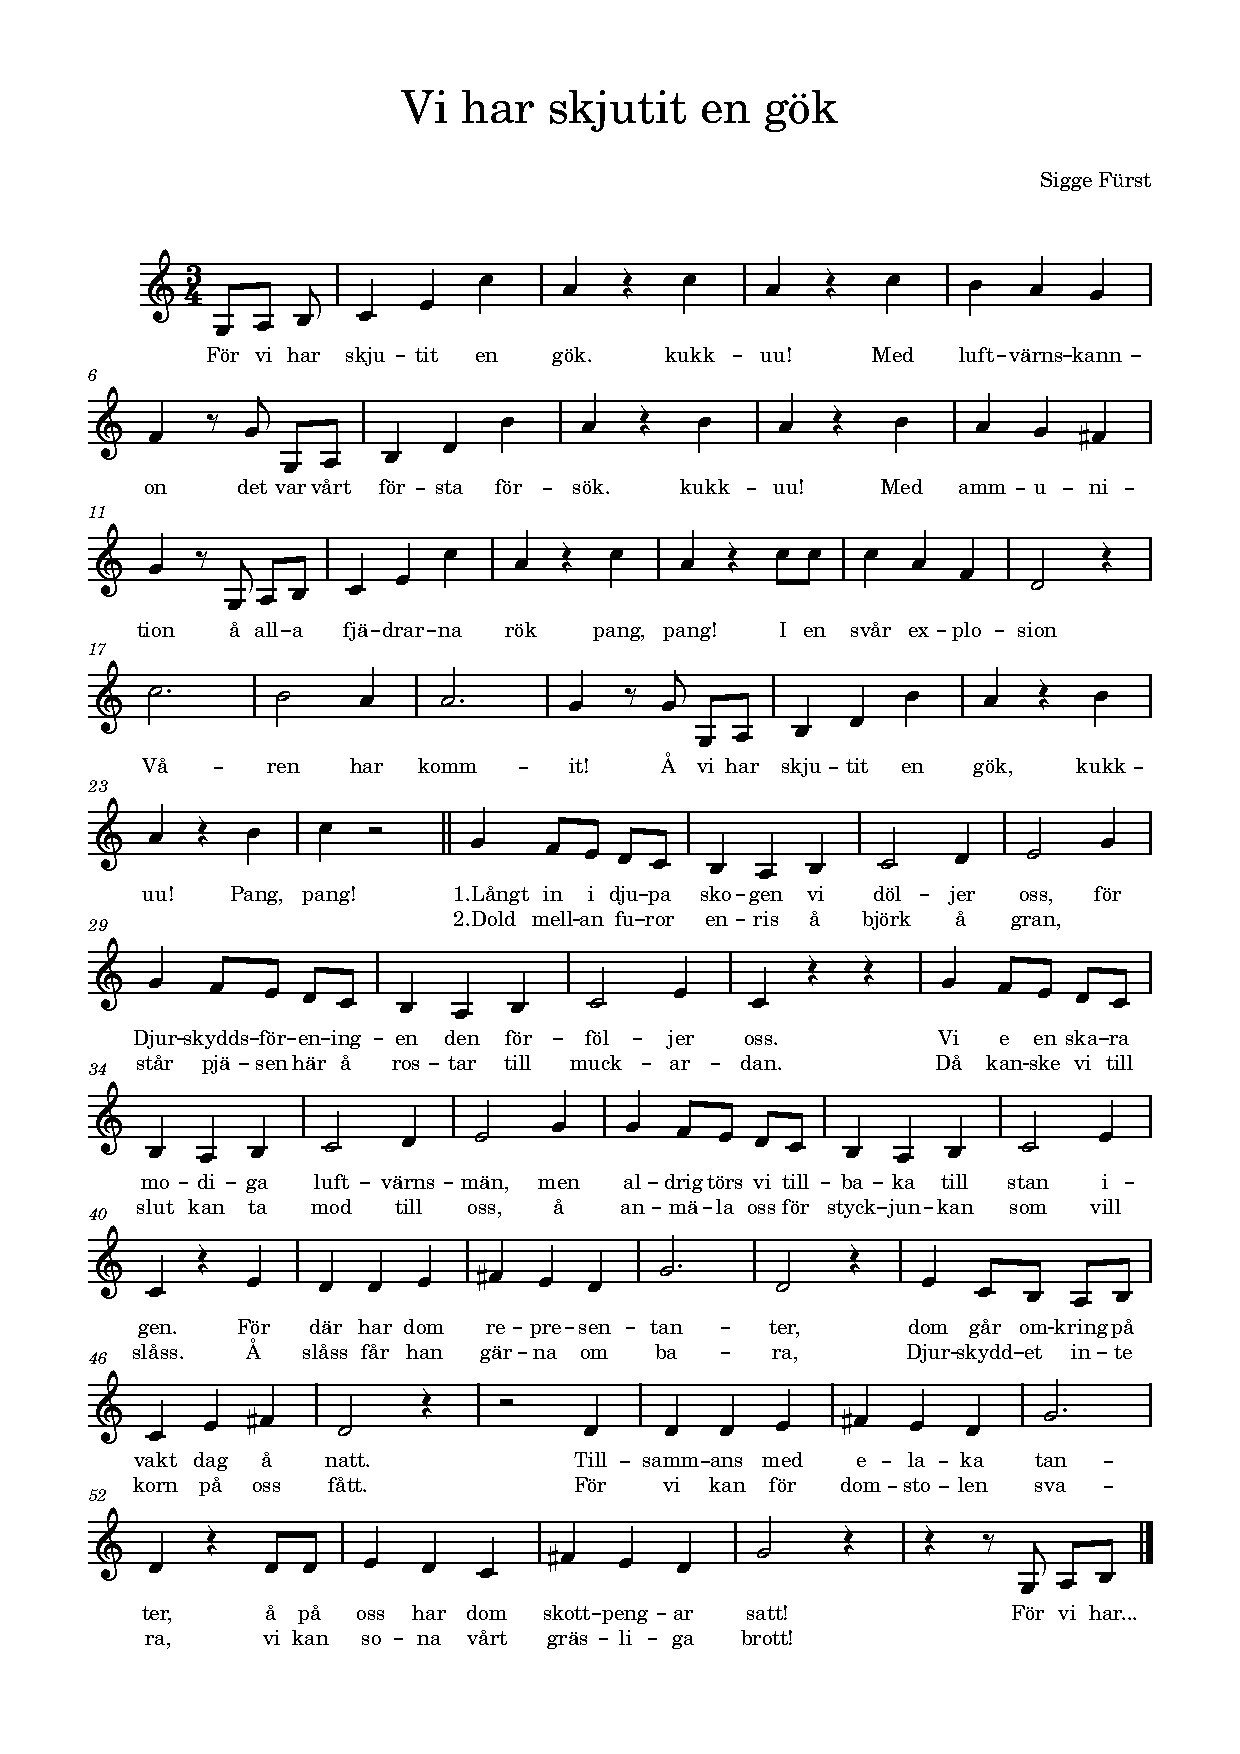
\includepdf[pages=-,pagecommand={},width=\textwidth]{Scores/skjutit_gok_not.pdf}

\newpage


\section*{2. En bit och en sup}
\paragraph*{John Hedéen}
$$$$
Ut till skärgården folket drar om i skärgårdsbåten dom flytit har\\
å att dom har skäl, det förstår man så väl.\\
Ja för där uti får man fisk å så får man luft som e salt å frisk\\
men den man får först de e törst!\\
Ja vet grannen breve, brukar vinkar mig ge,\\
ja han vinkar mig dit på en sup å en bit.\\
å ja säger ej nej, sen är turen hos mig,\\
han gör kontravisit på en sup å en bit.\\

\noindent
Besöken blir långa å suparna många,\\
så kulram behövs det för räkningens skull.\\
Man får hälsa så sund, å en mage så rund,\\
ja en härlig aptit av en sup å en bit.\\

\noindent
När man tagit sitt lilla dopp då ska rev å nätena plockas opp,\\
man sedan ett tag, över grynnan ror drag.\\
I en vassrugge strax intill sen ja låter ekan min ligga still,\\
ja tar en till knark i min ark!.\\
Etiketten är god, när det dukas ombord,\\
utan duk som är vit tas en sup å en bit.\\
Å så hör man ett skrik, ifrån Anderssons vik:\\
"Hörrudu titta hit på en sup å en bit".\\

\noindent
När sommarn är härlig är törsten besvärlig,\\
mera än vanligt så uppskattas då:\\
Orden frukost å mål, å naturligtvis 'Skål!'.\\
Som en prick över i:t är en sup å en bit.\\

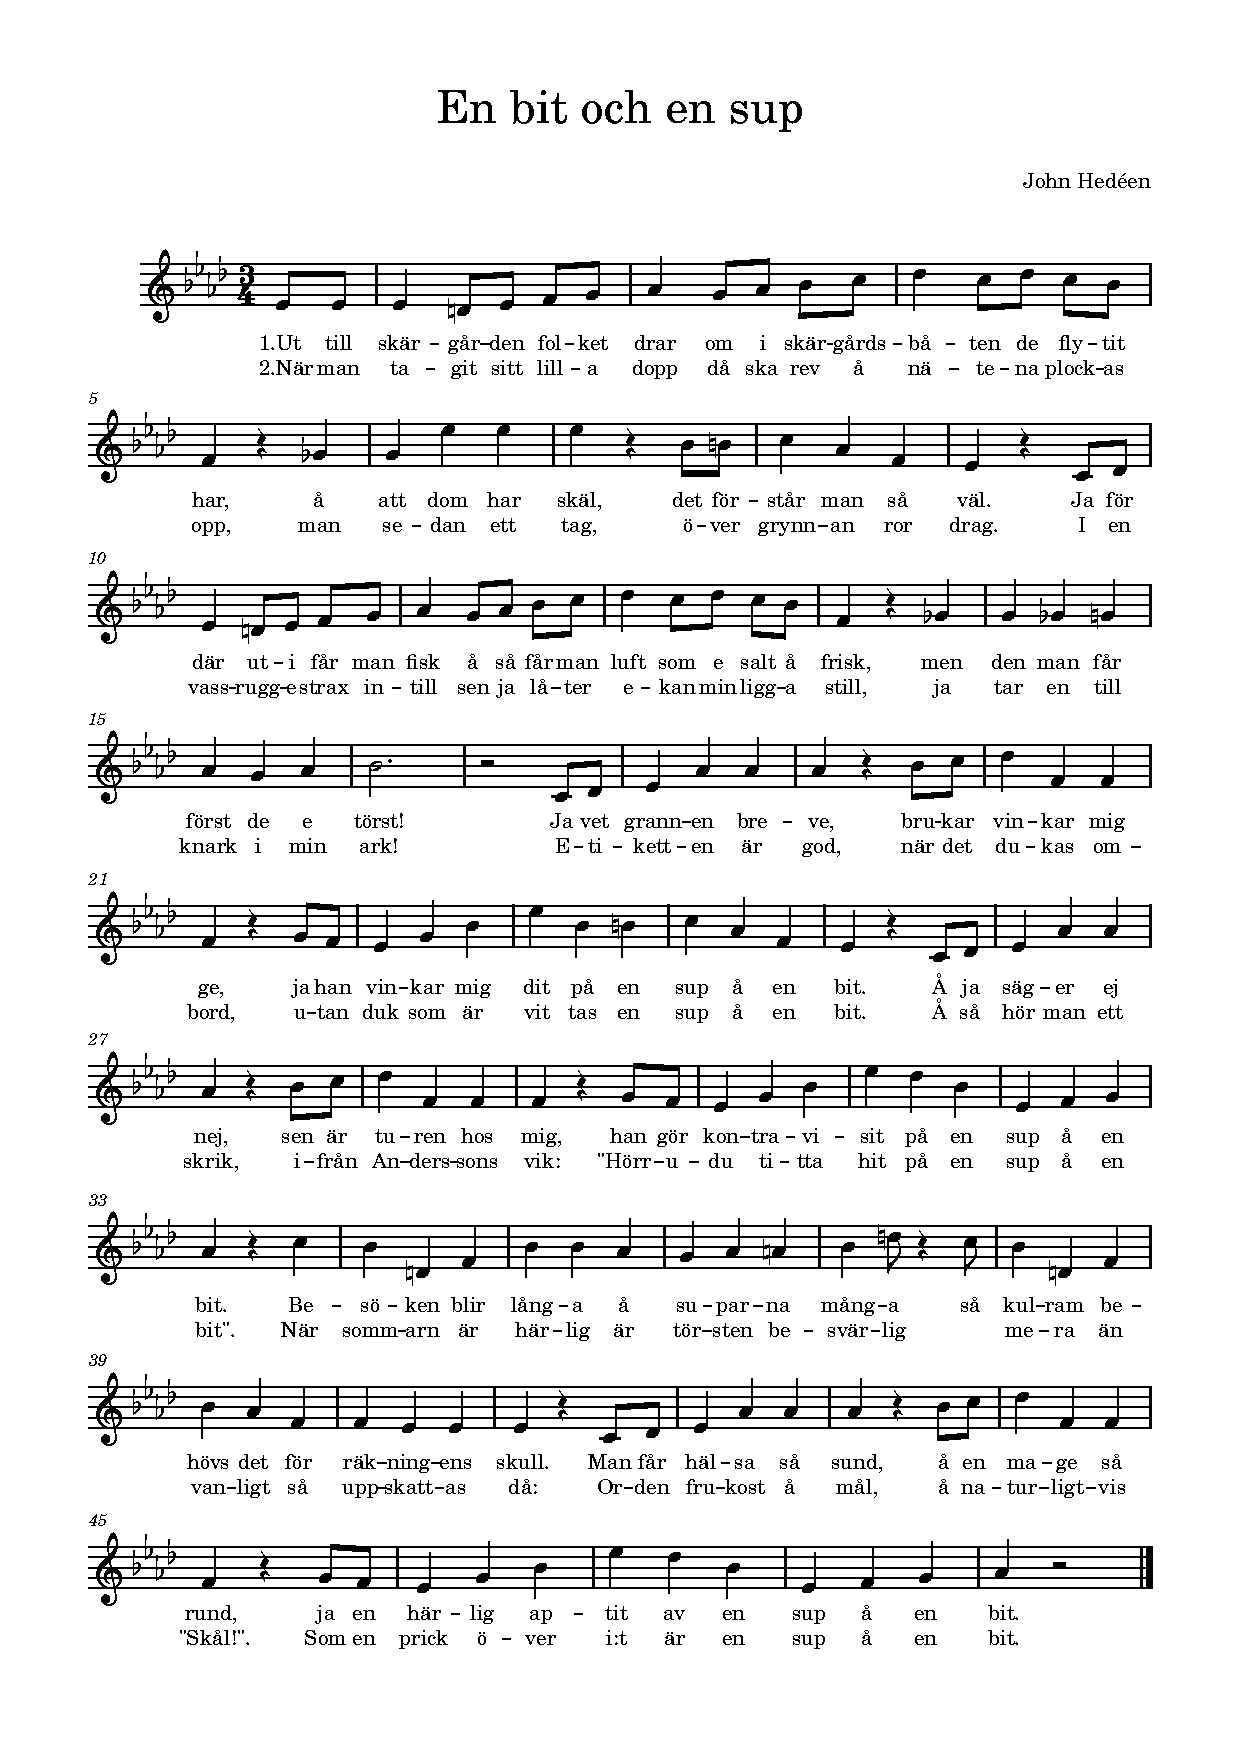
\includepdf[pages=-,pagecommand={},width=\textwidth]{Scores/En_bit_och_en_sup.pdf}

\newpage
\section*{3. Svettvisan}
\paragraph*{Bosse österberg}
$$$$
De sköna damerna svettas lätt uti barmen,\\
å blusen fuktas så smått i veck under armen.\\
så sant som dörren e som en del utav karmen,\\
så e odören liksom en del utav charmen.\\

\noindent
En herres svettning e mera våldsam å ymnig,\\
trots att nätskjortan hans e luftig å rymlig.\\
Ja lite svett gör de bara lätt när han joggar,\\
å vatten finns ju till för att få svalkande groggar.\\

\noindent
Den raska herrn å den sköna damen med vecket,\\
beslöt att pröva på lite svett under täcket.\\
Men fastän kärleken e båd döver å blinder,\\
så har den luktsinnet kvar som ställer till hinder.\\

\noindent
Så hör än hit, ni som e så heta på gröten,\\
å som besväras av vad som doftar från fötren.\\
Löp inte risk att vid sängen lämnas vid kanten,\\
håll på er skorna så har ni glädje av tanten.\\

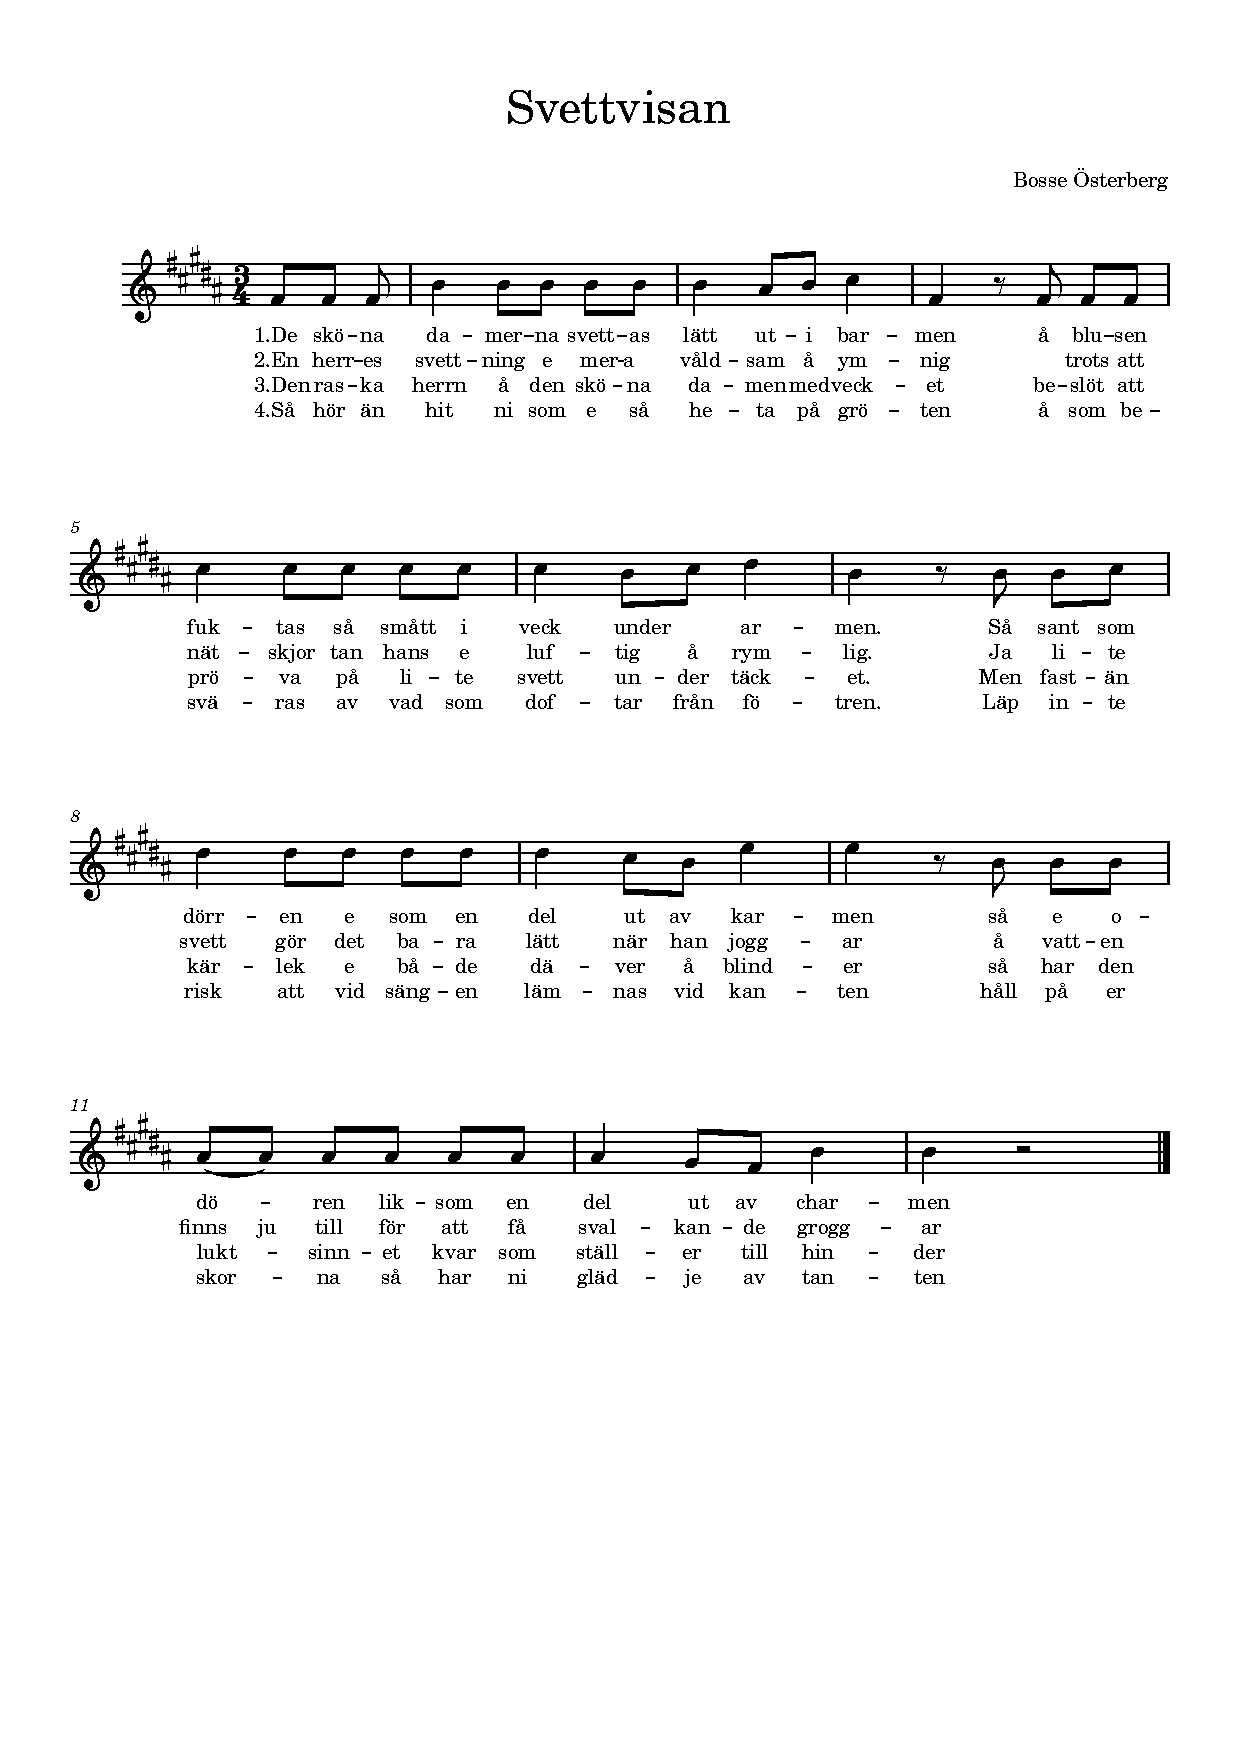
\includepdf[pages=-,pagecommand={},width=\textwidth]{Scores/Svettvisan.pdf}


\newpage
\noindent
\begin{minipage}{0.5\textwidth}
	\paragraph*{Lille Albin\\}
	\vspace{3px}
	\textit{Mel: Albertina}\\
\end{minipage}

\noindent
\begin{minipage}{0.45\textwidth}
	Där byggdes en maskot i Norden\\
	Lille Albin det var maskotens namn\\
	Musikprogram!\\

	\noindent
	Hopp' på Albin, må så vara\\
	Föll från Albin, ingen fara\\
	Lyss till Albins närradioprogram \\
	Festprogram!\\

	\noindent
	Lille Albin är allaredan målad\\
	Han är målad i svart och silvergrått\\
	Genombrott!\\

	\noindent
	Svart som natten, må så vara\\
	Tål ej vatten, ingen fara\\
	Hörs bland skratten och musik omlott\\
	Hemfridsbrott\\

	\noindent
	Lille Albin han är nu redan lastad\\
	Han är lastad med öl och brännevin\\
	Öl och vin!\\

	\noindent
	Första hjälpen, må så vara\\
	Ta' en käck en, ingen fara\\
	Njut av skvätten, en folkets medicin\\
	Medicin\\


\end{minipage}%
\hspace{0.05\textwidth}
\noindent
\begin{minipage}{0.45\textwidth}
	
	\noindent
	På gatorna bits Lille Albin\\
	Ja, han smak för akilleshälen har\\
	Blottad, bar!\\

	\noindent
	Ont i foten, må så vara\\
	Vi vet boten, ingen fara\\
	Ta' dig supen, så finns ej smärtan kvar\\
	Sen vi tar!\\

	\noindent
	Lille Albin har allaredan suckat\\
	Ja, han suckat sin sista melodi\\
	Hysteri!\\

	\noindent
	Tyst kring Albin, må så vara\\
	Fixa Albin, ingen fara\\
	Lyss till Albin, med nya batter i!\\
	Skadefri!\\

	\noindent
	Nu är allt som en gång det varit\\
	För alla runtom är han sig lik!\\
	Byggteknik/Magnifik!\\

	\noindent
	Biskopsgatan, må så vara\\
	och dess vänner, ingen fara\\
	Än har vi Albin, han äro änglalik\\
	Är sig lik!\\

	
\end{minipage}


\end{document}